
%%%%%%%%%%%%%%%%%%%%%%%%%%%%%%%%%%%%%%%%%
% Programming/Coding Assignment
% LaTeX Template
%
% This template has been downloaded from:
% http://www.latextemplates.com
%
% Original author:
% Ted Pavlic (http://www.tedpavlic.com)
%
% Note:
% The \lipsum[#] commands throughout this template generate dummy text
% to fill the template out. These commands should all be removed when 
% writing assignment content.
%
% This template uses a Perl script as an example snippet of code, most other
% languages are also usable. Configure them in the "CODE INCLUSION 
% CONFIGURATION" section.
%
%%%%%%%%%%%%%%%%%%%%%%%%%%%%%%%%%%%%%%%%%

%----------------------------------------------------------------------------------------
%	PACKAGES AND OTHER DOCUMENT CONFIGURATIONS
%----------------------------------------------------------------------------------------



\documentclass{article}

\usepackage{fancyhdr} % Required for custom headers
\usepackage{lastpage} % Required to determine the last page for the footer
\usepackage{extramarks} % Required for headers and footers
\usepackage[usenames,dvipsnames]{color} % Required for custom colors
\usepackage{graphicx} % Required to insert images
\usepackage{listings} % Required for insertion of code
\usepackage{courier} % Required for the courier font
\usepackage{lipsum} % Used for inserting dummy 'Lorem ipsum' text into the template
\usepackage{setspace}
\usepackage{color}
\usepackage{comment}
\usepackage{caption}
\usepackage[T1]{fontenc}
\usepackage{hyperref}
\usepackage{natbib}
\usepackage{underscore}
\usepackage{subfigure}
\usepackage{fixltx2e}

\hypersetup{
    colorlinks=true,
    linkcolor=blue,
    filecolor=magenta,      
    urlcolor=cyan,
    breaklinks=true
}

\usepackage[]{algorithm2e}
\usepackage{pdfpages}
\usepackage{tikz}




%For python inclusion (http://widerin.org/blog/syntax-highlighting-for-python-scripts-in-latex-documents)
\definecolor{Code}{rgb}{0,0,0}
\definecolor{Decorators}{rgb}{0.5,0.5,0.5}
\definecolor{Numbers}{rgb}{0.5,0,0}
\definecolor{MatchingBrackets}{rgb}{0.25,0.5,0.5}
\definecolor{Keywords}{rgb}{0,0,1}
\definecolor{self}{rgb}{0,0,0}
\definecolor{Strings}{rgb}{0,0.63,0}
\definecolor{Comments}{rgb}{0,0.63,1}
\definecolor{Backquotes}{rgb}{0,0,0}
\definecolor{Classname}{rgb}{0,0,0}
\definecolor{FunctionName}{rgb}{0,0,0}
\definecolor{Operators}{rgb}{0,0,0}
\definecolor{Background}{rgb}{0.98,0.98,0.98}

% Margins
\topmargin=-0.45in
\evensidemargin=0in
\oddsidemargin=0in
\textwidth=6.5in
\textheight=9.0in
\headsep=0.25in

\linespread{1.1} % Line spacing

% Set up the header and footer
\pagestyle{fancy}
\lhead{\hmwkAuthorName} % Top left header
\chead{\hmwkClass\ (\hmwkClassInstructor\ \hmwkClassTime): \hmwkTitle} % Top center head
\chead{\hmwkClass\ (\hmwkClassInstructor): \hmwkTitle} % Top center head
\rhead{\firstxmark} % Top right header
\lfoot{\lastxmark} % Bottom left footer
\cfoot{} % Bottom center footer
\rfoot{Page\ \thepage\ of\ \protect\pageref{LastPage}} % Bottom right footer
\renewcommand\headrulewidth{0.4pt} % Size of the header rule
\renewcommand\footrulewidth{0.4pt} % Size of the footer rule

\setlength\parindent{0pt} % Removes all indentation from paragraphs

%----------------------------------------------------------------------------------------
%	CODE INCLUSION CONFIGURATION
%----------------------------------------------------------------------------------------

\definecolor{MyDarkGreen}{rgb}{0.0,0.4,0.0} % This is the color used for comments
\lstloadlanguages{Perl} % Load Perl syntax for listings, for a list of other languages supported see: ftp://ftp.tex.ac.uk/tex-archive/macros/latex/contrib/listings/listings.pdf
\lstset{language=Perl, % Use Perl in this example
        frame=single, % Single frame around code
        basicstyle=\small\ttfamily, % Use small true type font
        keywordstyle=[1]\color{Blue}\bf, % Perl functions bold and blue
        keywordstyle=[2]\color{Purple}, % Perl function arguments purple
        keywordstyle=[3]\color{Blue}\underbar, % Custom functions underlined and blue
        identifierstyle=, % Nothing special about identifiers                                         
        commentstyle=\usefont{T1}{pcr}{m}{sl}\color{MyDarkGreen}\small, % Comments small dark green courier font
        stringstyle=\color{Purple}, % Strings are purple
        showstringspaces=false, % Don't put marks in string spaces
        tabsize=5, % 5 spaces per tab
        %
        % Put standard Perl functions not included in the default language here
        morekeywords={rand},
        %
        % Put Perl function parameters here
        morekeywords=[2]{on, off, interp},
        %
        % Put user defined functions here
        morekeywords=[3]{test},
       	%
        morecomment=[l][\color{Blue}]{...}, % Line continuation (...) like blue comment
        numbers=left, % Line numbers on left
        firstnumber=1, % Line numbers start with line 1
        numberstyle=\tiny\color{Blue}, % Line numbers are blue and small
        stepnumber=5 % Line numbers go in steps of 5
}

% Creates a new command to include a perl script, the first parameter is the filename of the script (without .pl), the second parameter is the caption
\newcommand{\perlscript}[2]{
\begin{itemize}
\item[]\lstinputlisting[caption=#2,label=#1]{#1.pl}
\end{itemize}
}


%----------------------------------------------------------------------------------------
%	DOCUMENT STRUCTURE COMMANDS
%	Skip this unless you know what you're doing
%----------------------------------------------------------------------------------------

% Header and footer for when a page split occurs within a problem environment
\newcommand{\enterProblemHeader}[1]{
\nobreak\extramarks{#1}{#1 continued on next page\ldots}\nobreak
\nobreak\extramarks{#1 (continued)}{#1 continued on next page\ldots}\nobreak
}

% Header and footer for when a page split occurs between problem environments
\newcommand{\exitProblemHeader}[1]{
\nobreak\extramarks{#1 (continued)}{#1 continued on next page\ldots}\nobreak
\nobreak\extramarks{#1}{}\nobreak
}

\setcounter{secnumdepth}{0} % Removes default section numbers
\newcounter{homeworkProblemCounter} % Creates a counter to keep track of the number of problems

\newcommand{\homeworkProblemName}{}
\newenvironment{homeworkProblem}[1][Problem \arabic{homeworkProblemCounter}]{ % Makes a new environment called homeworkProblem which takes 1 argument (custom name) but the default is "Problem #"
\stepcounter{homeworkProblemCounter} % Increase counter for number of problems
\renewcommand{\homeworkProblemName}{#1} % Assign \homeworkProblemName the name of the problem
\section{\homeworkProblemName} % Make a section in the document with the custom problem count
\enterProblemHeader{\homeworkProblemName} % Header and footer within the environment
}{
\exitProblemHeader{\homeworkProblemName} % Header and footer after the environment
}

\newcommand{\problemAnswer}[1]{ % Defines the problem answer command with the content as the only argument
\noindent\framebox[\columnwidth][c]{\begin{minipage}{0.98\columnwidth}#1\end{minipage}} % Makes the box around the problem answer and puts the content inside
}

\newcommand{\homeworkSectionName}{}
\newenvironment{homeworkSection}[1]{ % New environment for sections within homework problems, takes 1 argument - the name of the section
\renewcommand{\homeworkSectionName}{#1} % Assign \homeworkSectionName to the name of the section from the environment argument
\subsection{\homeworkSectionName} % Make a subsection with the custom name of the subsection
\enterProblemHeader{\homeworkProblemName\ [\homeworkSectionName]} % Header and footer within the environment
}{
\enterProblemHeader{\homeworkProblemName} % Header and footer after the environment
}

%----------------------------------------------------------------------------------------
%	NAME AND CLASS SECTION
%----------------------------------------------------------------------------------------

\newcommand{\hmwkTitle}{Assignment\ \#2 } % Assignment title
%\newcommand{\hmwkDueDate}{Monday,\ January\ 1,\ 2012} % Due date
\newcommand{\hmwkClass}{Web Science} % Course/class
%\newcommand{\hmwkClassTime}{10:30am} % Class/lecture time
\newcommand{\hmwkClassInstructor}{Alexander Nwala} % Teacher/lecturer
\newcommand{\hmwkAuthorName}{Puneeth Bikkasandra} % Your name

%----------------------------------------------------------------------------------------
%	TITLE PAGE
%----------------------------------------------------------------------------------------

\title{
\vspace{2in}
\textmd{\textbf{\hmwkClass:\ \hmwkTitle}}\\
%\normalsize\vspace{0.1in}\small{Due\ on\ \hmwkDueDate}\\
%\vspace{0.1in}\large{\textit{\hmwkClassInstructor\ \hmwkClassTime}}
\vspace{0.1in}\large{\textit{\hmwkClassInstructor}}
\vspace{3in}
}

\author{\textbf{\hmwkAuthorName}}
\date{Thursday, February 15, 2018} % Insert date here if you want it to appear below your name

%----------------------------------------------------------------------------------------

\begin{document}

\maketitle
\newpage



%----------------------------------------------------------------------------------------
%	TABLE OF CONTENTS
%----------------------------------------------------------------------------------------

%\setcounter{tocdepth}{1} % Uncomment this line if you don't want subsections listed in the ToC

\newpage
\tableofcontents
\newpage

%----------------------------------------------------------------------------------------
%	PROBLEM 1
%----------------------------------------------------------------------------------------

% To have just one problem per page, simply put a \clearpage after each problem

\begin{homeworkProblem}

Write a Python program that extracts 1000 unique links from Twitter. Omit links from the Twitter domain (twitter.com)\\
Also note that you need to verify that the final target URI (i.e.,the one that responds with a 200) is unique.  You could have many different shortened URIs for www.cnn.com (t.co, bit.ly, goo.gl,etc.).\\

%\problemAnswer{
 \textbf{SOLUTION :}\\
 
  
  \begin{enumerate}
  \item \textbf{} The program requires one to create the Twitter developer keys and access Tokens. Find the below process to obtain the keys and access tokens\\ \\
  \textbf{} 1. Creating an user account at "https://www.twitter.com" \\
  \textbf{} 2. Log in to "https://www.apps.twitter.com/" and create an application\\
	      	(note: The developer needs to fill the form found after clicking the "Create App" option)\\
   \textbf{} 3. Finally, selecting the "Generate secret access tokens" option will create the tokens, which could be used to call twitter APIs \\
		      
 \end{enumerate}
 
%\begin{figure}[h]
 % \centering
  %  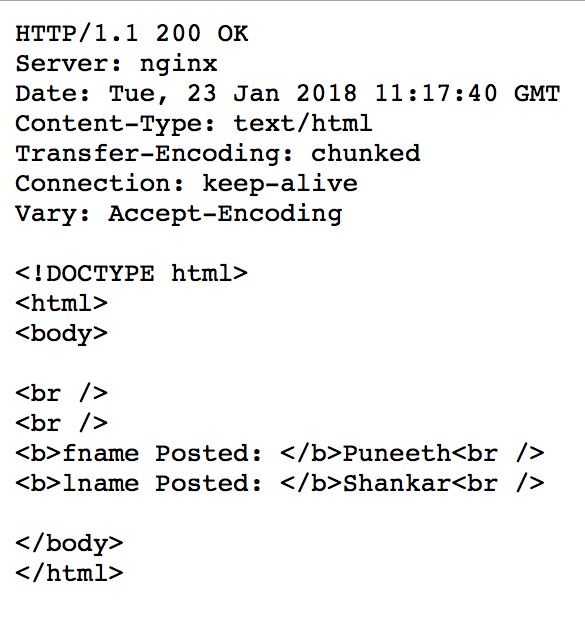
\includegraphics[width=0.5\textwidth]{webScience}
    %  \caption{Sample 'curl' with POST}
%\end{figure}
 
%}
\textbf{}Extracting 1000 unique links from the twitter feed across all the users worldwide :\\
   The below code in Listing 1; extracts the web links, captures the redirection and finally saves in an independent file.\\
  
\begin{lstlisting}[language=Python, caption=twitterLinks.py]

from tweepy.streaming import StreamListener
from tweepy import OAuthHandler
from tweepy import Stream
from BeautifulSoup import BeautifulSoup
from requests import Request, Session
import json
import time
import requests

ckey = 'L9QTLPWp2CswcJWRRaNtrsxWO'
csecret = 'nKm7PFmtFAWQYupqffdLz6YWD23VzFlNV8myAei7BaFYDNIoZN'
atoken = '962415725104324608-gJ39MDzaSIlbj44ZBSIuhezb3QcgOAx'
asecret = 'SD9uFFWZH5zfrg4taMdjXkH3vefgmqpPne10EmPiXLijg'
count = 0
uniqueLinks = set([])
linksFile = open("1000TwitterLinks.txt","w")

class listener(StreamListener):
	
	def on_data(self, data):
		global count
		if(count == 1300):
			return False
		else:	
			tweetJson = json.loads(data)
			username = tweetJson['user']['screen_name']
			links = tweetJson['entities']['urls']

			if( len(links) != 0 and tweetJson['truncated'] == False ):
				links = self.getLinksFromTweet(links)
		
				for link in links:
					global uniqueLinks,linksFile
					if(link in uniqueLinks):
						pass
					else:
						print(link)
						count = count + 1
						uniqueLinks.add(link)
						linksFile.write(link)
	     				linksFile.write('\n')	
			# time.sleep(1)				
		return True

	def getLinksFromTweet(self, linksDict):

		links = []
		destUrl = ''
		for uri in linksDict:

			if("https://twitter.com" in uri['expanded_url']):
				pass
			else:
				destUrl = self.checkForRedirection(uri['expanded_url'][0:])
				links.append(destUrl)

		return links

	def checkForRedirection(self,link1):
		response = requests.get(link1, verify=False, timeout=10)
		return response.url
		 	


	def on_error(self, status):
		if status == 420:
			#returning False in on_data disconnects the stream
			return False
		return True
	
	
auth = OAuthHandler(ckey, csecret)
auth.set_access_token(atoken, asecret)	
try:
	twitterStream = Stream(auth, listener())		
	twitterStream.filter(track=['football'])
except:
	twitterStream.filter(track=['football'])

\end{lstlisting}

\textbf{Sample listing of links obtained after extraction:}

\begin{lstlisting}[caption=Extracted Links]
https://www.nytimes.com/2018/02/11/opinion/head-trauma-football.html?partner=IFTTT
https://www.football-italia.net/117066/ht-benevento-shock-roma
https://mobile.twitter.com/ProSoccerSF/status/962740869999706112
https://paper.li/TibsNews/1359398292?edition_id=7f545270-0f6b-11e8-94d7-0cc47a0d164b
https://www.instagram.com/p/BfEfI8Ollhj/
https://www.kingfut.com/2018/02/11/kotoko-cara-three-penalty-misses/
https://www.change.org/p/save-youth-football-in-california
https://sportgid.net/football/levante-real-22-obzor-matcha-i-video-golov-03-02-2018/
http://football-station.net/b/2018/02/104384.html
http://www.football-chairman.com/
\end{lstlisting}

Remaining links can be found in the attached file \textbf{"1000twitterLinks.txt"}
\end{homeworkProblem}
\clearpage
\newpage

%----------------------------------------------------------------------------------------
%   PROBLEM 2
%----------------------------------------------------------------------------------------

\begin{homeworkProblem}
 
Download the TimeMaps for each of the target URIs.  We'll use the ODU Memento Aggregator,.\\
For example:\\

  \textbf{} URI-R = http://www.cs.odu.edu/ \\
   \textbf{} URI-T = http://memgator.cs.odu.edu/timemap/link/http://www.cs.odu.edu/ \\
     \textbf{} OR \\
   	\textbf{} URI-T = http://memgator.cs.odu.edu/timemap/json/http://www.cs.odu.edu/ \\
	
Create a histogram* of URIs vs. number of Mementos (as computed from the TimeMaps).  For example, 100 URIs with 0 Mementos, 300
URIs with 1 Memento, 400 URIs with 2 Mementos, etc.  The x-axis will have the number of mementos, and the y-axis will have the frequency
of occurance.\\
 
%\problemAnswer{
 \textbf{SOLUTION}\\\\
 The solution for this problem is outlined by the following steps:
 \begin{enumerate}
 \item \textbf{Passing the URL collected in a file "1000twitterLinks.txt" from previous code link in the following way:} 

 \begin{verbatim}
	http://memgator.cs.odu.edu/timemap/link/http://www.cs.odu.edu 
 \end{verbatim}
 
  \item \textbf{Extracting the timemap for each URI  :} The below code in Listing 1; extracts the time maps; Saves URI Index,URI Count and Mementos in an independent file.
 
\begin{lstlisting}[language=Python, caption=timeMaps.py]
import requests
import sys
import time

uri_t = "http://memgator.cs.odu.edu/timemap/link/" 
mementoList = []
plotMementosDict = {}
count = 1
headers = {'user-agent': 'my-app/0.0.1'}
f = open('1000TwitterLinks.txt','r')
fw = open('MemeFile.txt','w')
fw.write("Count,URI,Mementos")
fw.write('\n')
for line in f:
	if(line == ''):
		pass
	else:	
		response = requests.get(uri_t + line.strip(),headers=headers)
		print("...",response.status_code)
		if(response.status_code == 200):
			memento = response.headers['X-Memento-Count']
			mementoList.append(memento)
		else:
			mementoList.append(0)
		 
			

for value in mementoList:
	if(str(value) in plotMementosDict):
		uriValue = plotMementosDict.get(str(value))
		plotMementosDict[str(value)] = uriValue + 1
	else:
		uriValue = 0
		plotMementosDict[str(value)] = uriValue + 1
	
print("plotMementosDict : ",plotMementosDict)

for mementoValue in plotMementosDict:
	print('{:>8}  {:>8}'.format(str(plotMementosDict[mementoValue]),mementoValue))
	fw.write(str(count)+","+str(plotMementosDict[mementoValue])+","+
	str(mementoValue)) 
	fw.write("\n") 	
	count = count + 1

\end{lstlisting}
%}
TimeMaps obtained are saved in the format "Count,URI,Mementos" in to an independent text file as attached \textbf{"MemeFile.txt":}

\begin{lstlisting}[caption=Extracted TimeMaps]
Count,URI,Mementos
1,1,214
2,1,56
3,1,4183
4,1,36
5,1,131
6,1,136
7,1,6459
8,1,254
9,1,25
10,1,26
11,1,27
12,2,20
13,1,21
14,1,23
15,1,45
16,32,1
17,978,0
18,4,3
19,15,2
20,4,5
21,6,4
22,1,7
23,4,6
24,1,9
25,2,8
26,1,89917
27,1,4093
28,1,3488
29,1,77
30,1,32107
31,1,95
32,1,4778
33,1,13
34,1,12
35,1,2579
36,1,19
37,1,16
38,1,50
39,1,1472
40,1,49
41,1,295
\end{lstlisting}

\item \textbf{}The TimeMaps obtained are saved in CSV file and plotted as barplot . The below python code in Listing 5 creates a bargraph 

\begin{lstlisting}[language=Python, caption=histogram.py]
import matplotlib.pyplot as plt
import pandas as pd
import numpy as np

data=pd.read_csv('mem.csv', sep=',', skiprows=0,header=None, index_col =0).dropna() 
data.plot(kind='bar')
plt.ylim(0, 1000)
plt.ylabel("URIs")
plt.xlabel('mementos')
plt.title('Histogram')
L=plt.legend()
L.get_texts()[0].set_text('URIs')
plt.show()
\end{lstlisting}

The below graph shows the extracted content with \textbf{URI} at y-axis and \textbf{Mementos} at x-axis

\begin{figure}[h]
  \centering
    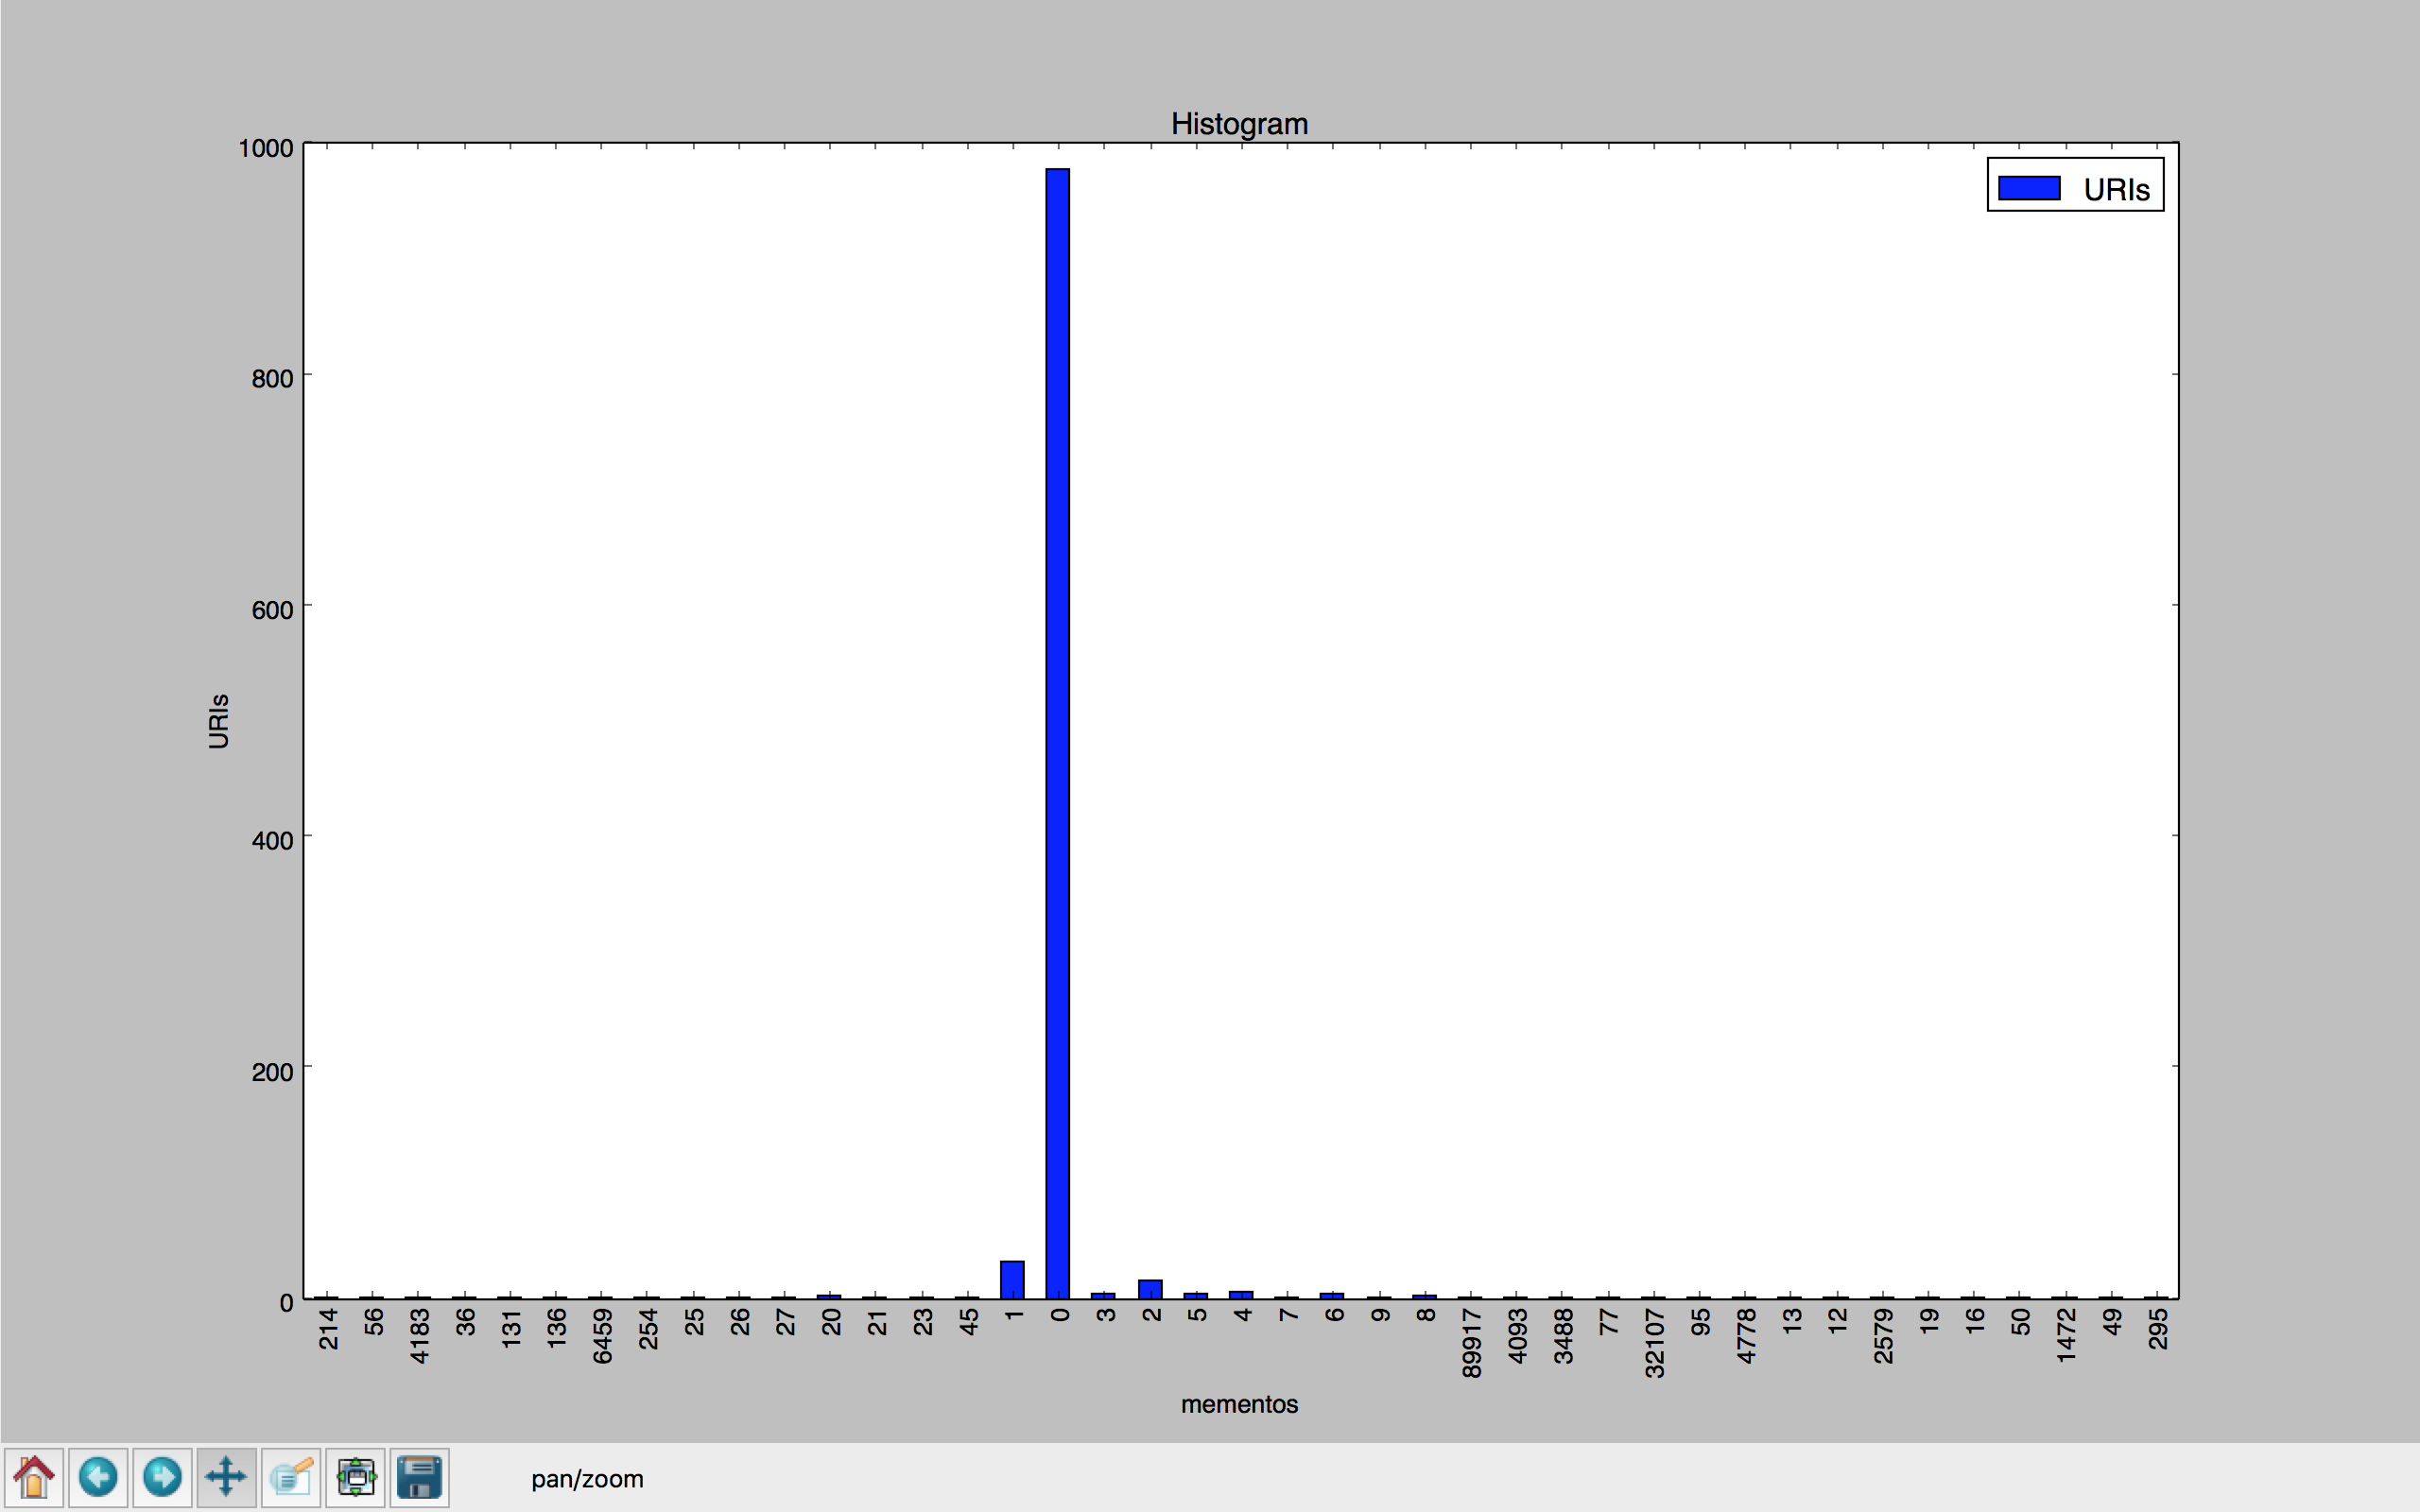
\includegraphics[width=0.5\textwidth]{histogram}
      \caption{Barplot URI vs  Mementos}
\end{figure}

\end{enumerate}


\end{homeworkProblem}
\clearpage
\newpage

%----------------------------------------------------------------------------------------
%   PROBLEM 3
%----------------------------------------------------------------------------------------

\begin{homeworkProblem}
Estimate the age of each of the 1000 URIs using the "Carbon Date" tool: \\
For URIs that have > 0 Mementos and an estimated creation date, create a graph with age 
(in days) on the x-axis and number of mementos on the y-axis.\\

Not all URIs will have Mementos, and not all URIs will have an estimated creation date.  \\Show how many fall into either categories.
For example,
\begin{verbatim}	
Total URIs:1000
Number of Mementos:137  
Number of Date Estimate:212
\end{verbatim}

%\problemAnswer{

 \textbf{SOLUTION}\\
Carbon Date for a site is calculated using the below URI pattern:

\begin{verbatim}
http://cd.cs.odu.edu/cd?url=http://www.cs.odu.edu/
\end{verbatim}

Where the above URL calculates the carbon date for "http://www.cs.odu.edu/"


\begin{lstlisting}[language=Python, caption=AgeMem.py]
import requests
import csv
import json
import sys
from datetime import datetime

noAge = 0
noMementos = 0
plotMementosDict = {}
totalURI = 0
f = open('1000TwitterLinks.txt','r')
for link in f:
	if(link == ''):
		pass
	else:
		try:
		totalURI = totalURI + 1
		carbonDateResponse = requests.get("http://cd.cs.odu.edu/cd/"+link)
		mementoResponse = requests.get("http://memgator.cs.odu.edu/
			timemap/json/"+link,stream=True,headers={'User-Agent': 'Mozilla/5.0'})
		print('Carbon Date status :',carbonDateResponse.status_code)
		print('Mementos status :',mementoResponse.status_code)
		carbonDateResponseJSON = carbonDateResponse.json()
		totalMementos = mementoResponse.headers["X-Memento-Count"]
		ageDate = carbonDateResponseJSON["estimated-creation-date"]

		if(ageDate == ""):
			noAge = noAge + 1
		if(totalMementos == '0'):
			noMementos = noMementos + 1

		print('No mementos: ', noMementos)
		print('No Carbon Date: ', noAge)

		if carbonDateResponse.status_code==200 and mementoResponse.status_code==200:
			now = datetime.now()
			createdDate = datetime.strptime(ageDate, '%Y-%m-%dT%H:%M:%S')
			currentAge = (now - createdDate)
			print('age: ', currentAge.days)
			print('Memento: ',totalMementos)
			plotMementosDict[str(currentAge.days)] = totalMementos

		except KeyboardInterrupt:
			exit()		
		except:
			print("An exception")
			pass

print('Total URIs',totalURI)
print('No Mementos',noMementos)
print('no date estimate',noAge)

with open('carbonDate.csv', 'wb') as csv_file:
	fieldsnames = ['currentAge','Mementos']
	writer = csv.DictWriter(csvfile, fieldnames=fieldsnames)
	writer.writeheader()
	# writer = csv.writer(csv_file)
	for age, MementoValue in plotMementosDict.items():
		writer.writerow({'currentAge': age, 'Mementos': MementoValue})
		# writer.writerow([age, MementoValue])	
				
\end{lstlisting}



     
   
%}

\end{homeworkProblem}
\clearpage
\newpage

\bibliographystyle{plain}
\bibliography{A1bibFile}

\end{document}
